\chapter{実装}
\label{implementation}

本章では提案手法の実装について述べる.

\section{実装環境}
\label{implementation:environment}
本節では,本研究で構築した実装環境について概説する.

\subsection{ハードウェアおよびソフトウェア}
\label{implementation:environment:resouces}

本研究で使用したハードウェアおよびソフトウェアとそのバージョンを以下に示す.

\begin{table}[htb]
  \begin{center}
    \caption{使用したハードウェアおよびソフトウェア}
    \begin{tabular}{|l|l|} \hline
      ハードウェア/ソフトウェア & 機種/バージョン \\ \hline
      Server & FUJITSU PRIMERGY S6 \\ \hline
      VMWare ESXi & 6.5 \\ \hline
      VyOS & 1.2.1 \\ \hline
      OpenVPN & 2.3.4 \\ \hline
      Ubuntu & 18.04 \\ \hline
      kubeadm & 1.16.3 \\ \hline
      kubelet & 1.16.3 \\ \hline
      kubectl & 1.16.3 \\ \hline
    \end{tabular}
  \end{center}
\end{table}

\subsection{物理サーバの準備}
\label{implementation:esxi}

本研究では、実装において複数のセグメントおよびKubernetesクラスタの構築に複数のサーバが必要であったため、それらを仮想的に作成できるVMWare ESXi(以下、ESXi)を導入した。
使用したのは、ESXi6.5だ。
ESXiはホストOSを必要とせず、直接ハードウェアにインストールさせて動作させるハイパーバイザー型であるため、まず初めにESXiインストーラの
ブータブルイメージをUSBメモリに書き込み、FUJITSUサーバにインストールした。
計二台のFUJITSUサーバにESXiをインストールし、それぞれ以下のIPアドレスを設定した。

\begin{table}[htb]
  \begin{center}
    \caption{ESXiのIPアドレス}
    \begin{tabular}{|l|l|} \hline
      名前 & IPアドレス \\ \hline
      1台目 & 10.4.0.13 \\ \hline
      2台目 & 10.4.0.14 \\ \hline
    \end{tabular}
  \end{center}
\end{table}

\subsection{ネットワーク構成}
\label{implementation:network-environment}

本節では、本研究で構築したネットワーク構成について説明する。

まず初めに、ESXiの仮想スイッチとVLANを用いて二つのESXiサーバ上に新たに計三つの論理セグメントを構築した。
Vlanによって論理的にセグメントを分割することで、お互いに通信不可能な環境とした。
以下に、Vlan IDと対応するアドレスプレフィックスを示す。
なお、元から存在する10.4.0.0/16のアドレスプレフィックスはVlan ID 0に対応している。

\begin{table}[htb]
  \begin{center}
    \caption{Vlan IDと対応するアドレスプレフィックス}
    \begin{tabular}{|l|l|} \hline
      Vlan ID & アドレスプレフィックス \\ \hline
      0 & 10.4.0.0/16 \\ \hline
      10 & 192.168.10.0/24 \\ \hline
      20 & 192.168.20.0/24 \\ \hline
      30 & 192.168.30.0/24 \\ \hline
    \end{tabular}
  \end{center}
\end{table}

\subsection{VMの準備}

ネットワーク構築後、Kubernetesクラスタの構築に必要なサーバをVMとして立ち上げた。
それぞれのVMのOSにはUbuntu18.04を採用した。
以下に構築したサーバの詳細を示す。

\begin{table}[htb]
  \begin{center}
    \caption{準備したVMの詳細}
    \begin{tabular}{|l|l|l|l|} \hline
      名前 & Vlan ID & IP & 役割 \\ \hline
      lb & 10 & 192.168.10.253 & マスターノードのロードバランサー \\ \hline
      master01 & 10 & 192.168.10.101 & マスターノード \\ \hline
      master02 & 10 & 192.168.10.102 & マスターノード \\ \hline
      master03 & 10 & 192.168.10.103 & マスターノード \\ \hline
      node01 & 20 & 192.168.20.101 & ワーカーノード \\ \hline
      node02 & 20 & 192.168.20.102 & ワーカーノード \\ \hline
      node03 & 30 & 192.168.30.101 & ワーカーノード \\ \hline
      node04 & 30 & 192.168.30.102 & ワーカーノード \\ \hline
    \end{tabular}
  \end{center}
\end{table}

\begin{table}[htb]
  \begin{center}
    \caption{OpenVPN設定前の各サーバの疎通性}
    \begin{tabular}{|c|c|c|c|c|c|c|c|} \hline
      & Master01 & Master02 & Master03 & Worker01 & Worker02 & Worker03 & Worker04 \\ \hline
      Master01 & \ & ○ & ○ & × & × & × & × \\ \hline
      Master02 & ○ & \ & ○ & × & × & × & × \\ \hline
      Master03 & ○ & ○ & \ & × & × & × & × \\ \hline
      Worker01 & × & × & × & \ & ○ & × & × \\ \hline
      Worker02 & × & × & × & ○ & \ & × & × \\ \hline
      Worker03 & × & × & × & × & × & \ & ○ \\ \hline
      Worker04 & × & × & × & × & × & ○ & \ \\ \hline
    \end{tabular}
  \end{center}
\end{table}

\begin{table}[htb]
  \begin{center}
    \caption{OpenVPN設定前の各サーバのIPアドレス}
    \begin{tabular}{|l|l|} \hline
      名前 & IPアドレス \\ \hline
      Master01 & 192.168.10.101 \\ \hline
      Master02 & 192.168.10.102 \\ \hline
      Master03 & 192.168.10.103 \\ \hline
      Worker01 & 192.168.20.101 / 10.23.1.2 \\ \hline
      Worker02 & 192.168.20.102 / 10.23.1.3 \\ \hline
      Worker03 & 192.168.30.101 / 10.23.1.4 \\ \hline
      Worker04 & 192.168.30.102 / 10.23.1.5 \\ \hline
    \end{tabular}
  \end{center}
\end{table}

\begin{table}[htb]
  \begin{center}
    \caption{OpenVPN設定前の各サーバの疎通性}
    \begin{tabular}{|c|c|c|c|c|c|c|c|} \hline
      & Master01 & Master02 & Master03 & Worker01 & Worker02 & Worker03 & Worker04 \\ \hline
      Master01 & \ & ○ & ○ & ○ & ○ & ○ & ○ \\ \hline
      Master02 & ○ & \ & ○ & ○ & ○ & ○ & ○ \\ \hline
      Master03 & ○ & ○ & \ & ○ & ○ & ○ & ○ \\ \hline
      Worker01 & ○ & ○ & ○ & \ & ○ & ○ & ○ \\ \hline
      Worker02 & ○ & ○ & ○ & ○ & \ & ○ & ○ \\ \hline
      Worker03 & ○ & ○ & ○ & ○ & ○ & \ & ○ \\ \hline
      Worker04 & ○ & ○ & ○ & ○ & ○ & ○ & \ \\ \hline
    \end{tabular}
  \end{center}
\end{table}

\subsection{Kubernetesクラスタ構成}
\label{implementation:kubernetes-environment}
本研究で構築したKubernetesクラスタは,クラスタを操作するマスターノード三台,コンテナ型アプリケーションを配置するワーカーノード六台によって構成される.
今回は,異なるセグメントに配置したマスターノードとワーカーノードでクラスタリングを行うことで,ネットワーク上で論理的に離れた環境下のステージング環境が
構築可能であることを示した.

~\ref{implementation:network-environment}で示したネットワーク構成とKubernetesクラスタ構成をまとめた表を以下に示す.

\section{システム全体}
\label{implementation:system}
本研究で構築した実装環境の図を以下に示す.

\begin{figure}[htbp]
  \begin{center}
    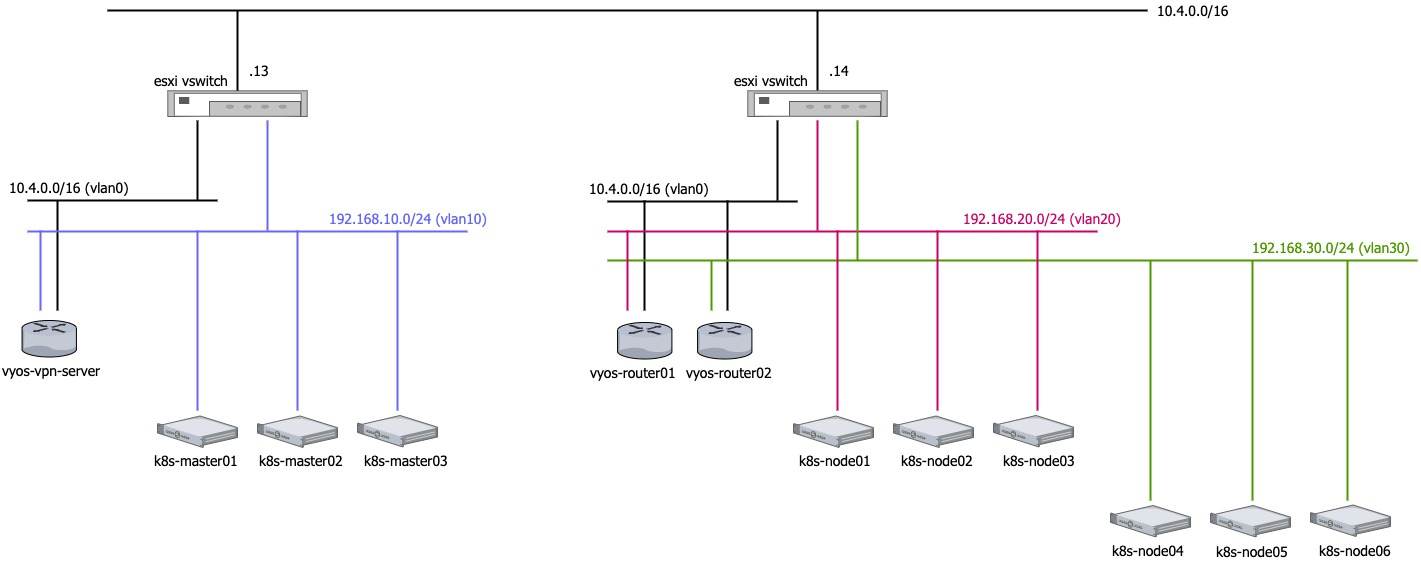
\includegraphics[width=\textwidth]{./figures/network-diagram.jpg}
    \caption{ネットワーク構成図}
  \end{center}
\end{figure}

%%% Local Variables:
%%% mode: japanese-latex
%%% TeX-master: "../bthesis"
%%% End:
